
%--------------------------------------
% Create title frame
\titleframe

%--------------------------------------
% Table of contents
%\begin{frame}{Overview}
%  \setbeamertemplate{section in toc}[sections numbered]
%  \tableofcontents
%\end{frame}

%--------------------------------------
% --- Slide 2: Review ---
\begin{frame}{You Have Learned}
    \begin{itemize}
        \item What is a microgrid (structure)
        \item What are its main components
        \item Power electronics interfaces (MPPT, etc.)
        \item The levels of control
%        \item How to make some forecasts
        \item How to design an installation using SMA’s software
    \end{itemize}
\end{frame}

% --- Slide 3: New Objectives ---
\begin{frame}{Optimal Control and Sizing}

    \textbf{Objective:} Learn how to optimally size and control a microgrid.
    
    We will still focus on a one-node microgrid for illustration

    \vspace{0.3cm}
    Possible problem extensions:
    \begin{itemize}
        \item \textbf{Microgrid networks:} Adding power flow equations (spatial complexity).
        \item \textbf{Multi-energy systems:} District heating, Hydrogen ($H_2$), etc..
        \item \textbf{Community microgrids:} Fairness and sharing considerations.
    \end{itemize}
\end{frame}

% --- Slide 4: Real-time Control (Animated) ---
\begin{frame}{Real-time Control:}

\begin{columns}
    \begin{column}{0.5\textwidth}
        \begin{center}
        \begin{tikzpicture}[node distance=2cm, auto, >=stealth, thick, scale=0.8, every node/.style={scale=0.8}]
            % Nodes
            \node[] (grid) {
\includegraphics[width=1cm]{images/utility-pole.png}};
            \node[below=0.2cm of grid, font=\scriptsize] {Public Grid};
            \node[circle, draw, right=2cm of grid] (sum) {\Large $+$};
            \node[right=1.5cm of sum, inner sep=5pt] (house) {
\includegraphics[width=1cm]{images/home.png}}; 
            \node[below=1.5cm of sum] (pv) {
\includegraphics[width=1cm]{images/PV.png}};
            
            % PV Flow (Dynamic)
            \draw[->] (pv) -- node[right] {
                \only<1-2>{6.3 kW}
                \only<3->{1.0 kW}
            } (sum);

            % House Flow (Dynamic)
            \draw[->] (sum) -- node[above] {
                \only<1-3>{0.7 kW}
                \only<4->{4.5 kW}
            } (house);

            % Grid Flow (Dynamic Direction and Value)
            % State 1: Exporting 5.6
            \draw<1>[<-] (grid) -- node[above] {5.6 kW} (sum);
            \draw<2>[<-] (grid) -- node[above] {0 kW} (sum);
            % State 3: PV drops, House 0.7, EV 7 -> Need 6.7kW from grid (Import)
            \draw<3>[->] (grid) -- node[above] {5.3 kW} (sum);
            % State 4: Consumption rises to 4.5 -> Need (4.5 + 7 - 1) = 10.5kW
            \draw<4->[->, very thick, red] (grid) -- node[above] {10.5 kW} (sum);

            % EV Node (Appears from step 2)
            \node<1->[above=1.5cm of sum] (ev) {
\includegraphics[width=1cm]{images/electric-car.png}};
            \draw<2->[->] (sum) -- node[left] {7.0 kW} (ev);
            
        \end{tikzpicture}
        \end{center}
    \end{column}

    \begin{column}{0.45\textwidth}
        Max grid exchange: \textbf{11.0 kW} \\ 
        \textbf{Sequence of events:}
        \begin{enumerate}
            \item<1-> Initial: Surplus exported to grid.
            \item<2-> \textbf{Car connects}: Adding 7 kW load.
            \item<3-> \textbf{Cloud passes}: PV drops to 1 kW.
            \item<4-> \textbf{Peak load}: House rises to 4.5 kW.
        \end{enumerate}
        
        \vspace{0.5cm}
        \only<4->{
            \begin{alertblock}{Decision Point}
                Import is at 10.5 kW. Any small increase will trip the 11 kW limit. 
                \textbf{Should you stop charging? }
            \end{alertblock}
        }
    \end{column}
\end{columns}
\end{frame}

% --- Slide 5: Operational Planning ---
\begin{frame}{Operational Planning (E.g. 24h ahead)}

    \begin{columns}
    \begin{column}{0.3\textwidth}
        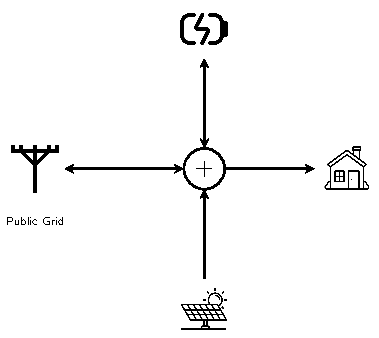
\includegraphics[width=\textwidth]{images/OP_system.pdf}
    \end{column}
    \begin{column}{0.6\textwidth}
        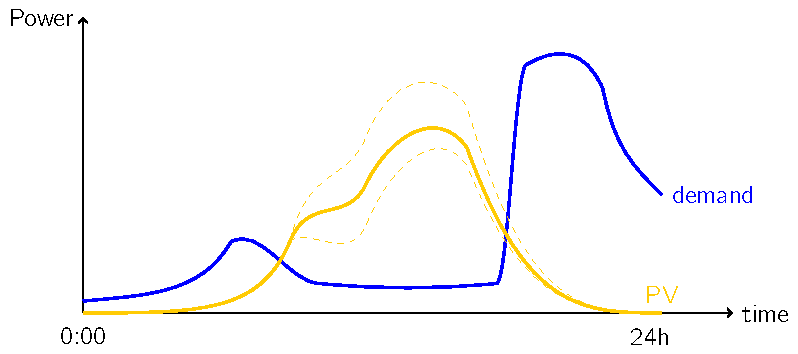
\includegraphics[width=\textwidth]{images/forecasts.pdf}\\
    \end{column}
    \end{columns}

\begin{itemize}
    \item Based on \textbf{forecasted demand and PV generation}.
    \item \textbf{Decisions:} Store, send back to grid, or move load?
    \item \textbf{Variables:} Function of prices, physical limits, and efficiencies.
\end{itemize}
\end{frame}

% --- Slide 6: Sizing ---
\begin{frame}{Sizing (Investment Decisions)}
    Strategic investment questions:
    \begin{itemize}
        \item Should you connect to the grid? Which power?
        \item Should you buy a genset or a CHP (Combined Heat and Power)?
        \item Should you invest in PV or wind generation?
        \item Should you invest in storage?
    \end{itemize}
    \vspace{0.5cm}
    \begin{alertblock}{Interdependence}
        Sizing decisions depend directly on the operational planning policy.
    \end{alertblock}
\end{frame}

% --- Slide 7: Hierarchical Coordination ---
\begin{frame}{Coordination of Time Scales}
    The global problem is decoupled in practice:
    \begin{table}
        \centering
        \begin{tabular}{|l|l|}
            \hline
            \textbf{Horizon} & \textbf{Decision Type} \\ \hline
            Yearly & Investment (Sizing) \\ \hline
            Hours/Days & Planning (Operational Planning) \\ \hline
            Minutes/Seconds & Adjustment (Real-time Control) \\ \hline
        \end{tabular}
    \end{table}
    \vspace{0.3cm}
    \centering
\end{frame}

\begin{frame} {Example: coordination between real-time control and operational planning}
\begin{columns}
  \begin{column}{0.5\textwidth}
    \begin{center}
        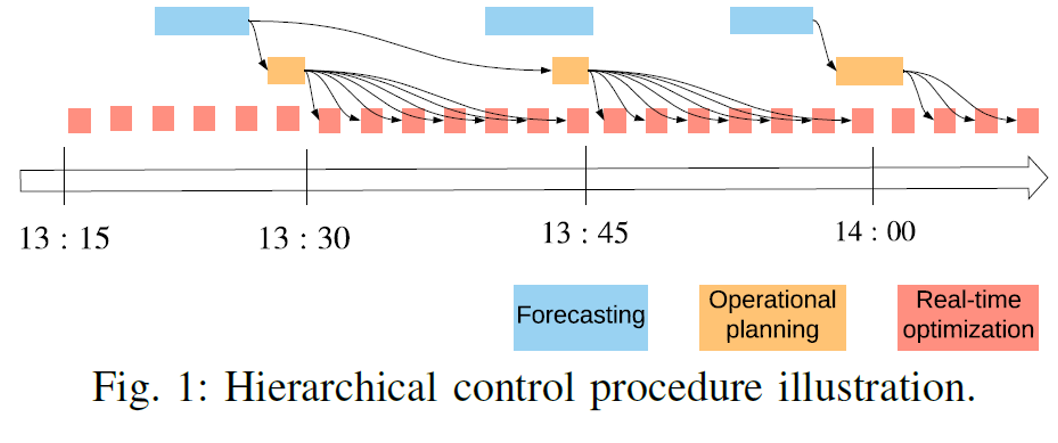
\includegraphics[width=\textwidth]{images/coordination_planning_RT.png}
    \end{center}  
  \end{column}
  \begin{column}{0.4\textwidth}
    {\footnotesize References: 
    \begin{itemize}
        \item Dumas, J., Dakir, S., Liu, C., \& Cornélusse, B. (2021). Coordination of operational planning and real-time optimization in microgrids. Electric Power Systems Research, 190, 106634.
        \item Moureau, C., Stegen, T., Glavic, M., \& Cornélusse, B. (2025). A Predictive Flexibility Aggregation Method for Low Voltage Distribution System Control. ORBi-University of Liège.
    \end{itemize}}
  \end{column}
\end{columns}


\end{frame}


\begin{frame} {Goals of this module}
    \begin{itemize}
        \item Learn about mathematical programming
        \item Learn to model problems as LPs or MIPs
        \item Understand how solvers work
        \item Solve the real-time control problem
        \item Learn to make some forecasts
        \item Solve the operational planning problem
        \item Solve the sizing problem
    \end{itemize}
\end{frame}

